% Compile with: latexmk -pdf synthid_reading_group.tex
% Alternatively, run pdflatex twice to populate the contents and slide count.
% Paper: https://www.nature.com/articles/s41586-024-08025-4
% Skeleton: title page, contents, and one empty frame per section.
% Suggested speaking time: 45 minutes, excluding questions and discussion.

\documentclass[aspectratio=169,11pt]{beamer}

% --------------------
% Theme (plain/minimal)
% --------------------
\usetheme{Boadilla}
\usecolortheme{seahorse}
\setbeamertemplate{blocks}[rounded][shadow=false]
\setbeamertemplate{navigation symbols}{}
\setbeamertemplate{footline}[frame number]

\AtBeginSection[]
{
    \begin{frame}
        \centering
        \vfill
        {\usebeamerfont{title}\usebeamercolor[fg]{title}\insertsectionhead\par}
        \vfill
    \end{frame}
}

% --------------------
% Packages
% --------------------
\usefonttheme{serif}
\usepackage[T1]{fontenc}
\usepackage[utf8]{inputenc}
\usepackage{newtxtext,newtxmath}
\usepackage{amsmath,amssymb}
\usepackage{graphicx}
\usepackage{booktabs}
\usepackage{caption}
\usepackage{bbm}

\hypersetup{
  colorlinks=true,
  urlcolor=blue,      % \url and \href external links
  linkcolor=blue,     % internal links (refs, TOC)
  citecolor=blue      % \cite links
}

\newcommand{\xl}[1]{\textcolor{brown}{[XL: #1]}}
\newcommand{\key}[1]{\textbf{#1}}
\newcommand{\focus}[1]{\textcolor{orange!80!black}{#1}}
\newcommand{\gray}[1]{\textcolor{gray}{#1}}
\renewcommand{\footnoterule}{}
\newcommand{\sourcenote}[1]{%
  \begingroup
  \renewcommand{\thefootnote}{}%
  \footnotetext{\tiny{#1}}%
  \endgroup
}
\newcommand{\ind}{\mathbbm{1}}

% Letters: bold symbols
\def\bA{\mathbf{A}}
\def\bB{\mathbf{B}}
\def\bC{\mathbf{C}}
\def\bD{\mathbf{D}}
\def\bE{\mathbf{E}}
\def\bF{\mathbf{F}}
\def\bG{\mathbf{G}}
\def\bH{\mathbf{H}}
\def\bI{\mathbf{I}}
\def\bJ{\mathbf{J}}
\def\bK{\mathbf{K}}
\def\bL{\mathbf{L}}
\def\bM{\mathbf{M}}
\def\bN{\mathbf{N}}
\def\bO{\mathbf{O}}
\def\bP{\mathbf{P}}
\def\bQ{\mathbf{Q}}
\def\bR{\mathbf{R}}
\def\bS{\mathbf{S}}
\def\bT{\mathbf{T}}
\def\bU{\mathbf{U}}
\def\bV{\mathbf{V}}
\def\bW{\mathbf{W}}
\def\bX{\mathbf{X}}
\def\bY{\mathbf{Y}}
\def\bZ{\mathbf{Z}}

\def\ba{\mathbf{a}}
\def\bb{\mathbf{b}}
\def\bc{\mathbf{c}}
\def\bd{\mathbf{d}}
\def\be{\mathbf{e}}
\def\bff{\mathbf{f}}
\def\bg{\mathbf{g}}
\def\bh{\mathbf{h}}
\def\bi{\mathbf{i}}
\def\bj{\mathbf{j}}
\def\bk{\mathbf{k}}
\def\bl{\mathbf{l}}
\def\bm{\mathbf{m}}
\def\bn{\mathbf{n}}
\def\bo{\mathbf{o}}
\def\bp{\mathbf{p}}
\def\bq{\mathbf{q}}
\def\br{\mathbf{r}}
\def\bs{\mathbf{s}}
\def\bt{\mathbf{t}}
\def\bu{\mathbf{u}}
\def\bv{\mathbf{v}}
\def\bw{\mathbf{w}}
\def\bx{\mathbf{x}}
\def\by{\mathbf{y}}
\def\bz{\mathbf{z}}

\def\bmu{\boldsymbol{\mu}}
\def\bbeta{\boldsymbol{\beta}}
\def\btheta{\boldsymbol{\theta}}
\def\bepsilon{\boldsymbol{\epsilon}}

\def\balph{\mathbf{\alpha}}
\def\bnu{\mathbf{\nu}}
\def\bbeta{\mathbf{\beta}}
\def\bxi{\mathbf{\xi}}
\def\bXi{\mathbf{\Xi}}
\def\bgam{\mathbf{\gamma}}
\def\bGam{\mathbf{\Gamma}}
\def\bdel{\mathbf{\delta}}
\def\bDel{\mathbf{\Delta}}
\def\bpi{\mathbf{\pi}}
\def\bPi{\mathbf{\Pi}}
\def\beps{\mathbf{\epsilon}}
\def\bveps{\mathbf{\varepsilon}}
\def\brho{\mathbf{\rho}}
\def\bvrho{\mathbf{\varrho}}
\def\bzeta{\boldsymbok{\zeta}}
\def\bsig{\mathbf{\sigma}}
\def\bSig{\mathbf{\Sigma}}
\def\bseta{\mathbf{\eta}}
\def\btau{\mathbf{tau}}
\def\btheta{\mathbf{\theta}}
\def\bvtheta{\mathbf{\vartheta}}
\def\bTheta{\mathbf{\Theta}}
\def\bupsilon{\mathbf{\upsilon}}
\def\bUpsilon{\mathbf{\Upsilon}}
\def\bphi{\mathbf{\phi}}
\def\bvphi{\mathbf{\varphi}}
\def\bPhi{\mathbf{\Phi}}
\def\bkappa{\mathbf{\kappa}}
\def\bchi{\mathbf{\chi}}
\def\blambda{\mathbf{\lambda}}
\def\bLambda{\mathbf{\Lambda}}
\def\bpsi{\mathbf{\psi}}
\def\bPsi{\mathbf{\Psi}}
\def\bmu{\mathbf{\mu}}
\def\bomega{\mathbf{\omega}}
\def\bOmega{\mathbf{\Omega}}
\def\bepsilon{\mathbf{\epsilon}}
\def\bdelta{\mathbf{\delta}}

\def\bzero{\mathbf{0}}
\def\bone{\mathbf{1}}

% Letters: blackboard font
\def\A{\mathbb{A}}
\def\B{\mathbb{B}}
\def\C{\mathbb{C}}
\def\D{\mathbb{D}}
\def\E{\mathbb{E}}
\def\F{\mathbb{F}}
\def\G{\mathbb{G}}
\def\H{\mathbb{H}}
\def\I{\mathbb{I}}
\def\J{\mathbb{J}}
\def\K{\mathbb{K}}
\def\L{\mathbb{L}}
\def\M{\mathbb{M}}
\def\N{\mathbb{N}}
\def\O{\mathbb{O}}
\def\P{\mathbb{P}}
\def\Q{\mathbb{Q}}
\def\R{\mathbb{R}}
\def\S{\mathbb{S}}
\def\T{\mathbb{T}}
\def\U{\mathbb{U}}
\def\V{\mathbb{V}}
\def\W{\mathbb{W}}
\def\X{\mathbb{X}}
\def\Y{\mathbb{Y}}
\def\Z{\mathbb{Z}}

\def\a{\mathbb{a}}
\def\b{\mathbb{b}}
\def\c{\mathbb{c}}
\def\d{\mathbb{d}}
\def\e{\mathbb{e}}
\def\f{\mathbb{f}}
\def\g{\mathbb{g}}
\def\h{\mathbb{h}}
\def\i{\mathbb{i}}
\def\j{\mathbb{j}}
\def\k{\mathbb{k}}
\def\l{\mathbb{l}}
\def\m{\mathbb{m}}
\def\n{\mathbb{n}}
\def\o{\mathbb{o}}
\def\p{\mathbb{p}}
\def\q{\mathbb{q}}
\def\r{\mathbb{r}}
\def\s{\mathbb{s}}
\def\t{\mathbb{t}}
\def\u{\mathbb{u}}
\def\v{\mathbb{v}}
\def\w{\mathbb{w}}
\def\x{\mathbb{x}}
\def\y{\mathbb{y}}
\def\z{\mathbb{z}}

% Letters: caligraphics
\def\cA{\mathcal{A}}
\def\cB{\mathcal{B}}
\def\cC{\mathcal{C}}
\def\cD{\mathcal{D}}
\def\cE{\mathcal{E}}
\def\cF{\mathcal{F}}
\def\cG{\mathcal{G}}
\def\cH{\mathcal{H}}
\def\cI{\mathcal{I}}
\def\cJ{\mathcal{J}}
\def\cK{\mathcal{K}}
\def\cL{\mathcal{L}}
\def\cM{\mathcal{M}}
\def\cN{\mathcal{N}}
\def\cO{\mathcal{O}}
\def\cP{\mathcal{P}}
\def\cQ{\mathcal{Q}}
\def\cR{\mathcal{R}}
\def\cS{\mathcal{S}}
\def\cT{\mathcal{T}}
\def\cU{\mathcal{U}}
\def\cV{\mathcal{V}}
\def\cW{\mathcal{W}}
\def\cX{\mathcal{X}}
\def\cY{\mathcal{Y}}
\def\cZ{\mathcal{Z}}

% Moment operators
\newcommand{\mean}{\mathbb{E}}
\newcommand{\Var}{\text{\rm Var}}
\newcommand{\Cov}{\text{\rm Cov}}

% Stochastic convergence and equality
\newcommand{\darrow}{\xrightarrow{\;\text{\tiny\rm d}\;}}
\newcommand{\parrow}{\xrightarrow{\;\text{\tiny\rm p}\;}}
\newcommand{\equdist}{\stackrel{\text{\rm\tiny d}}{=}}
\newcommand{\equas}{=_{\text{\rm\tiny a.s.}}}

% Curly braces in various sizes
\newcommand{\braces}[1]{{\lbrace #1 \rbrace}}
\newcommand{\bigbraces}[1]{{\bigl\lbrace #1 \bigr\rbrace}}
\newcommand{\Bigbraces}[1]{{\Bigl\lbrace #1 \Bigr\rbrace}}
\newcommand{\biggbraces}[1]{{\biggl\lbrace #1 \biggr\rbrace}}
\newcommand{\Biggbraces}[1]{{\Biggl\lbrace #1 \Biggr\rbrace}}

% Drawn iid from...
\DeclareMathOperator{\simiid}{\sim_{\mbox{\tiny iid}}}

% Various math operators in smaller sizes
\DeclareMathOperator{\tsum}{{\textstyle\sum}}
\DeclareMathOperator{\tprod}{{\textstyle \prod}}
\DeclareMathOperator{\msum}{\medmath\sum}
\DeclareMathOperator{\mprod}{\medmath\prod}
\DeclareMathOperator{\mint}{\scaleobj{.8}{\int}}
\DeclareMathOperator*{\medcup}{\raisebox{-.15em}{$\mathbin{\scalebox{1.5}{\ensuremath{\cup}}}$}}
\DeclareMathOperator*{\medcap}{\raisebox{-.15em}{$\mathbin{\scalebox{1.5}{\ensuremath{\cap}}}$}}

% argmax, argmin, conditional independence symbol
\DeclareMathOperator{\argmax}{\text{\rm argmax}}
\DeclareMathOperator{\argmin}{\text{\rm argmin}}
\DeclareMathOperator{\condind}{{\perp\!\!\!\perp}}

% Minimal styling. Beamer loads hyperref automatically.
% \usetheme{default}
\usefonttheme{professionalfonts}
\definecolor{navy}{RGB}{31,58,95}
\setbeamercolor{structure}{fg=navy}
\setbeamercolor{title}{fg=navy}
\setbeamercolor{frametitle}{fg=navy}
\setbeamertemplate{navigation symbols}{}
% \setbeamertemplate{footline}[frame number]
\setbeamertemplate{section in toc}[sections numbered]


% Edit presenter details and add the scheduled presentation date here.
\title[Scalable text watermarking]{Scalable watermarking for identifying large language model outputs}
\subtitle{Dathathri et al., \textit{Nature} (2024)}
\author{Xing Liu}
\institute{QuantCo reading group}
\date{7 Oct 2026}

\begin{document}

% Front page
\begin{frame}[plain]
    \titlepage
\end{frame}

% Table of contents updates automatically from the sections below.
\begin{frame}{Contents}
    \tableofcontents[hideallsubsections]
\end{frame}

\section{Motivation}
\begin{frame}[t]{Motivation}
    \begin{figure}
        \centering
        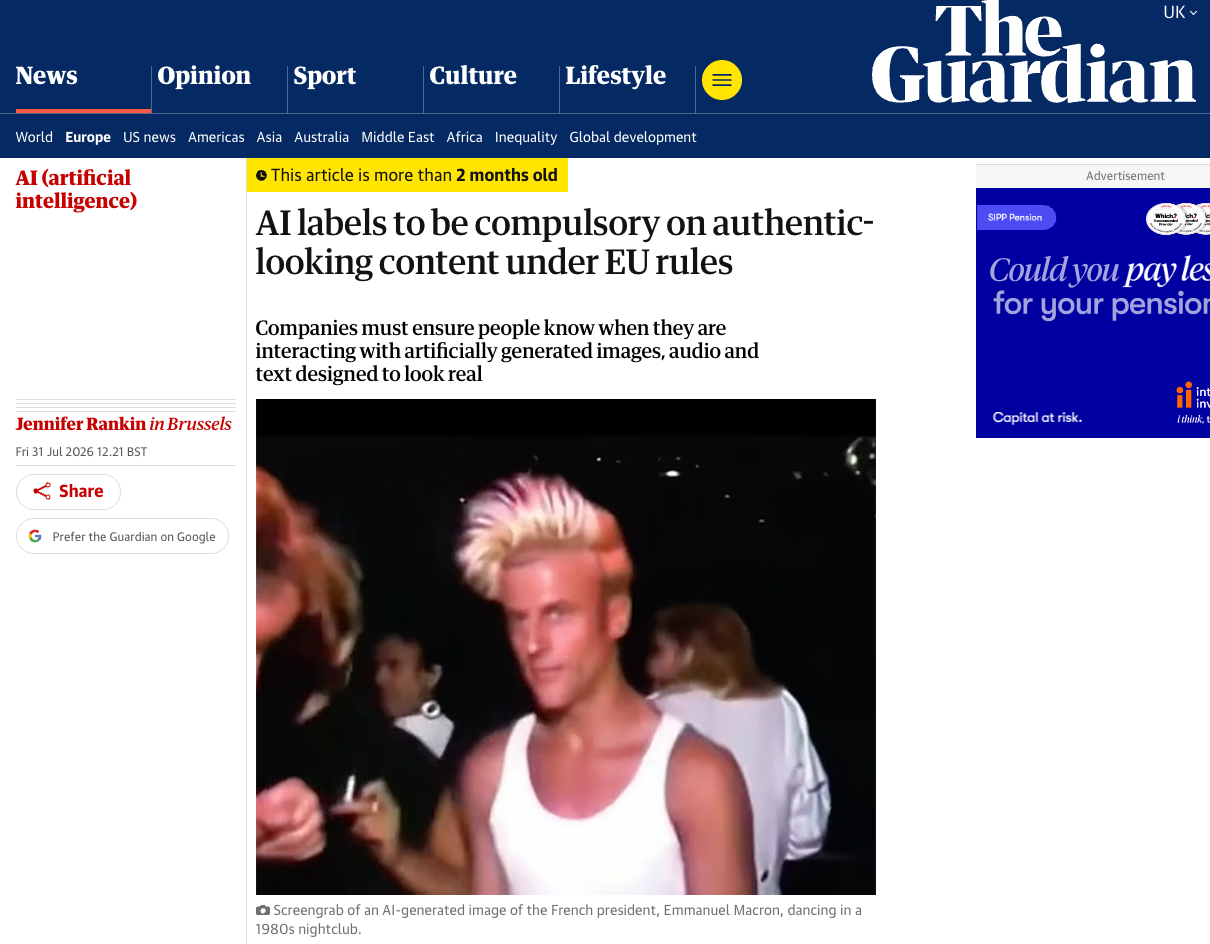
\includegraphics[width=0.5\textwidth]{figs/motivation_macron.png}
        \caption*{\href{https://www.theguardian.com/technology/2026/jul/31/ai-labels-to-be-compulsory-on-authentic-looking-content-under-eu-rules}{Link.} EU AI Act enforcement, starting from 2nd August 2026.}
    \end{figure}
\end{frame}

\begin{frame}[t]{Motivation}
    \begin{figure}
        \centering
        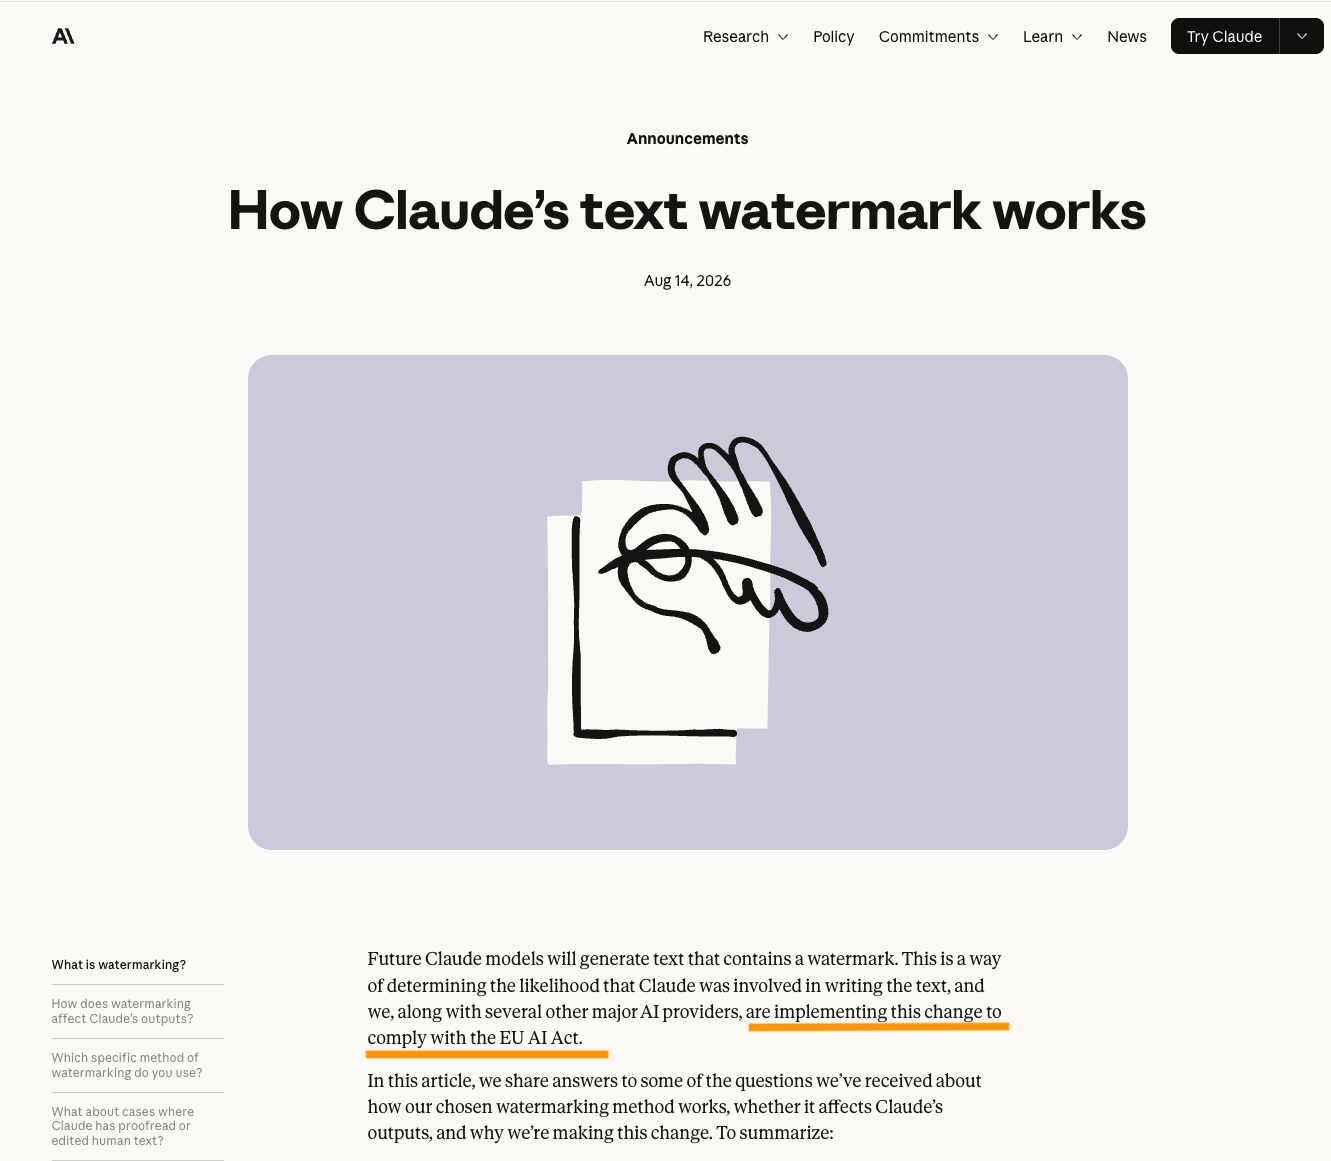
\includegraphics[width=0.5\textwidth]{figs/motivation_anthropic.png}
        \caption*{\href{https://www.anthropic.com/news/claude-text-watermark}{Link.} Anthropic adopts text watermarking.}
    \end{figure}
\end{frame}

\begin{frame}[t]{Motivation}
    \begin{figure}
        \centering
        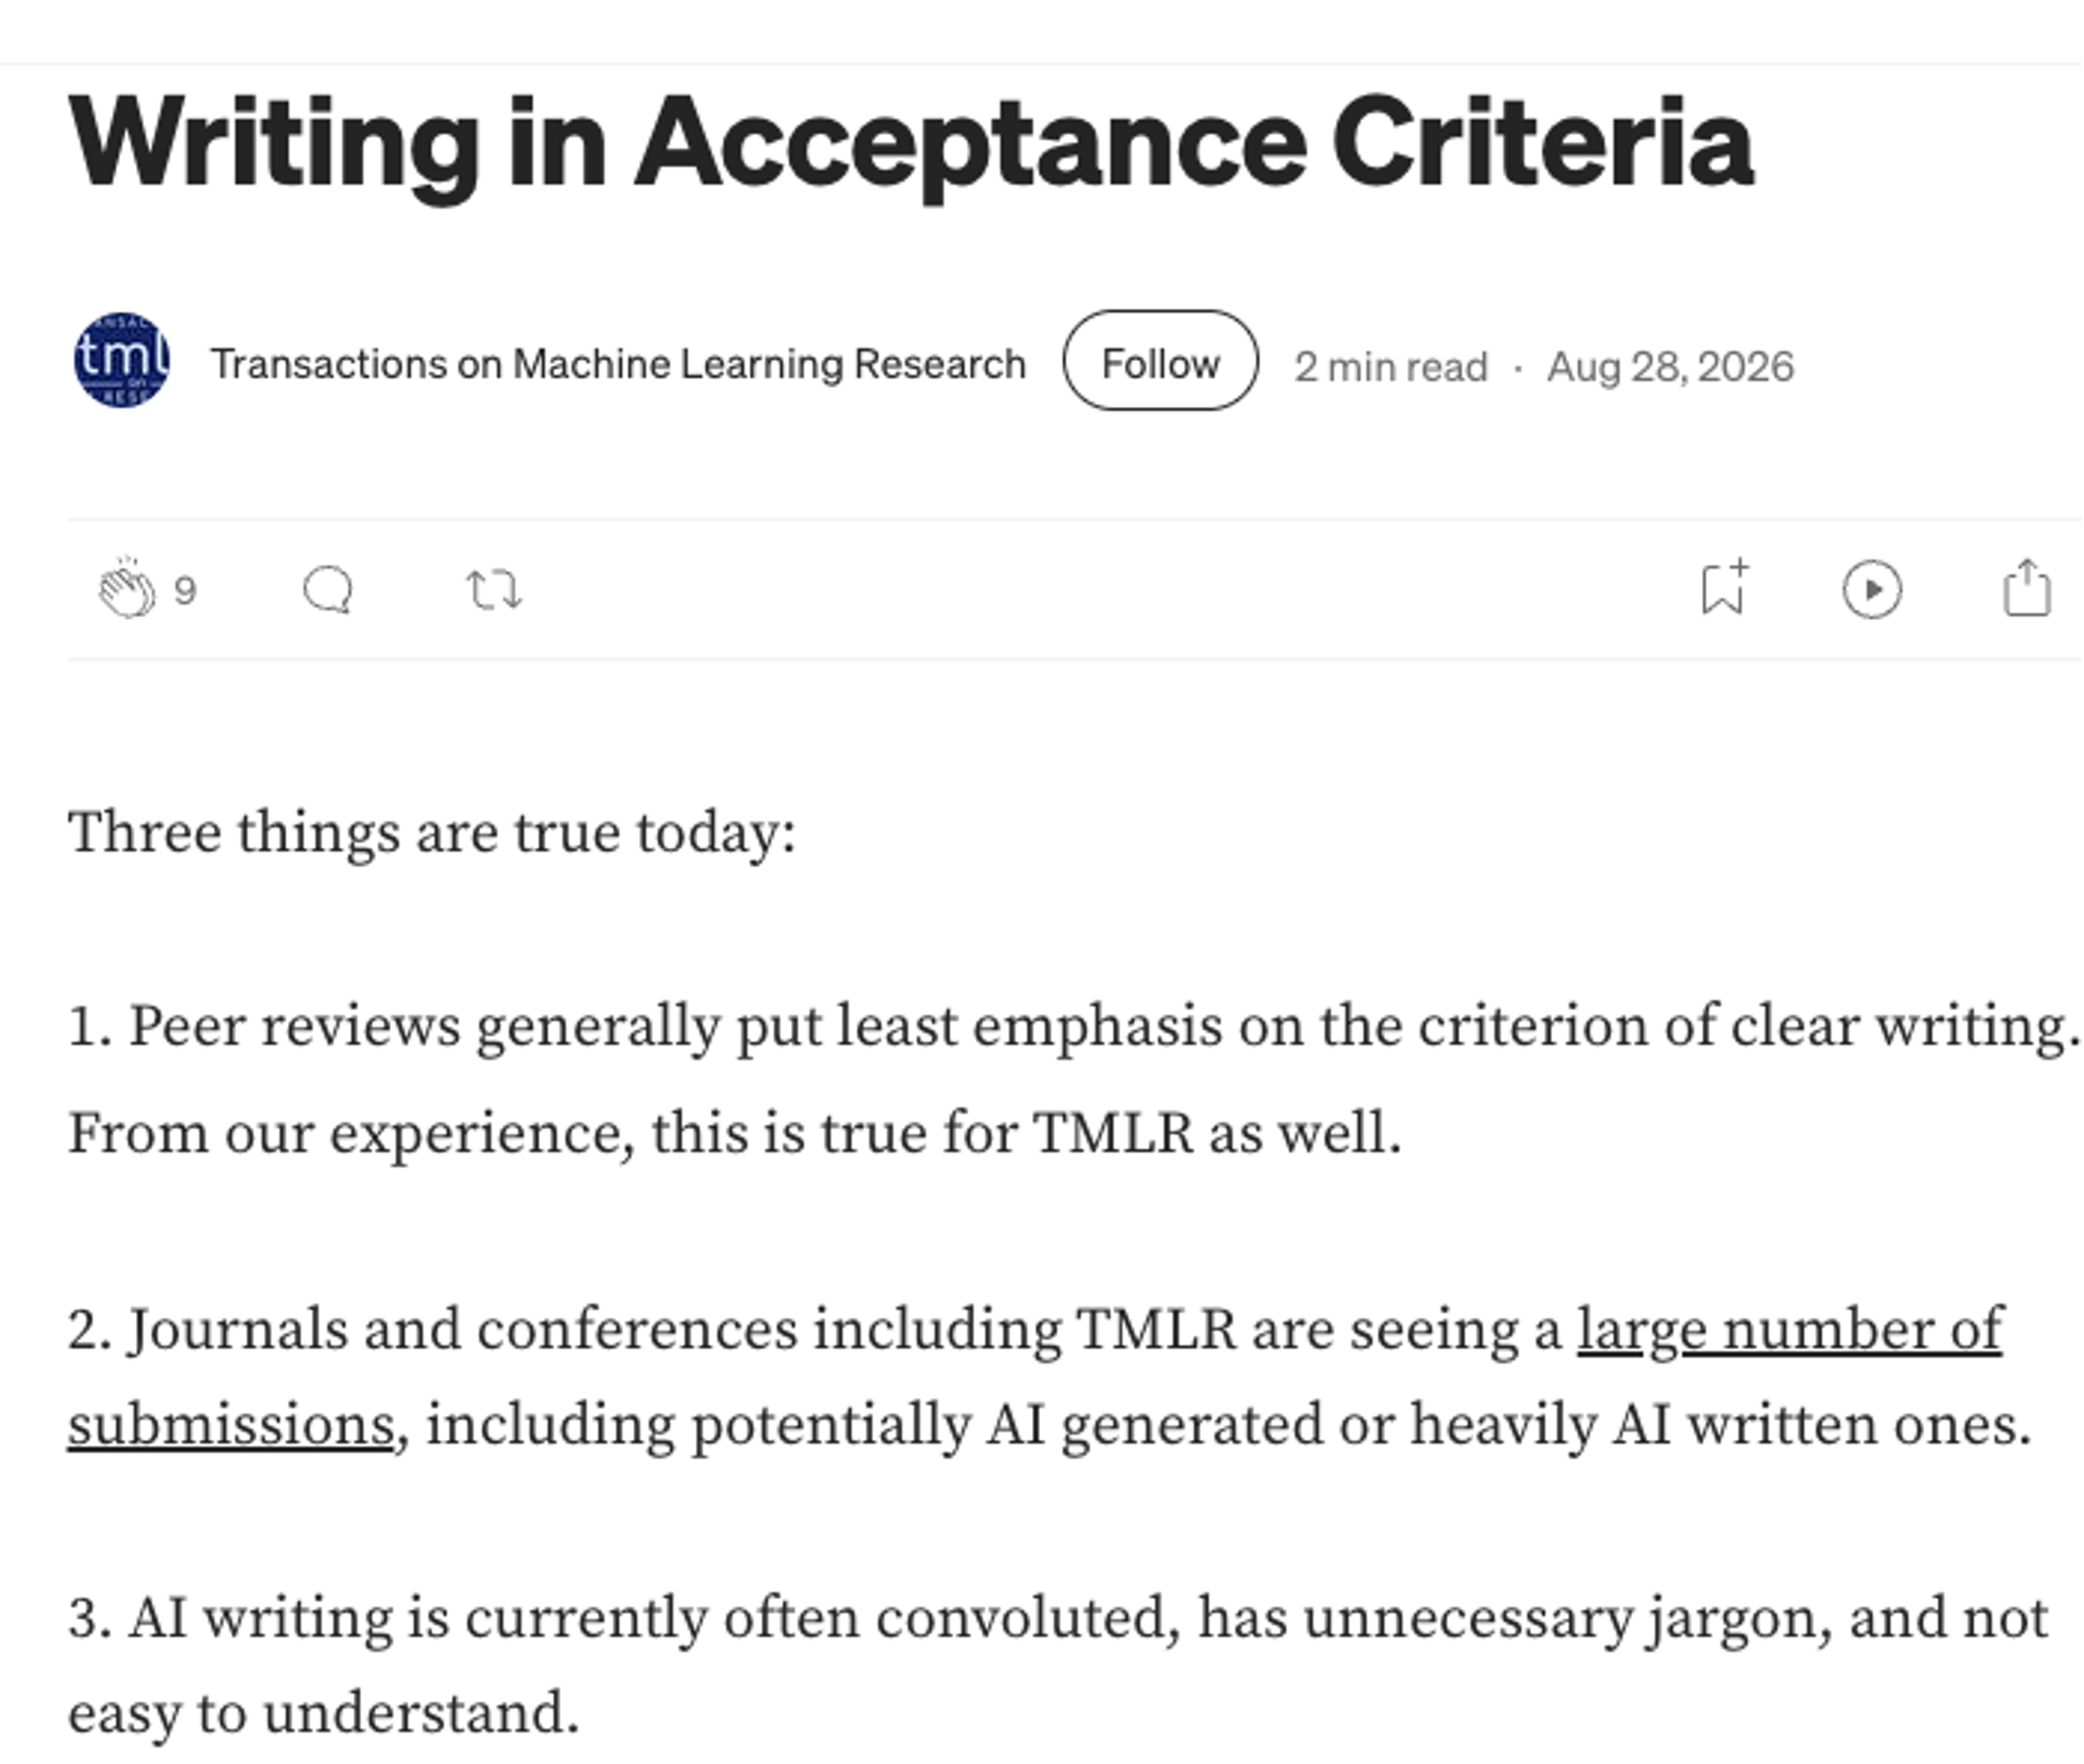
\includegraphics[width=0.5\textwidth]{figs/motivation_tmlr.png}
        \caption*{\href{https://medium.com/@TmlrOrg/increasing-emphasis-on-clear-writing-in-acceptance-criteria-bfd75349f5e9}{Link.} TMLR's call for reviewers to emphasise more on clarity of writing due to surges in AI-generated content.}
    \end{figure}
\end{frame}

\section{Background}
\begin{frame}[t]{How LLMs Generate Texts}
    \begin{itemize}
        \item Most LLMs generate text using autoregressive next-token sampling.
    \end{itemize}
    \begin{figure}
        \centering
        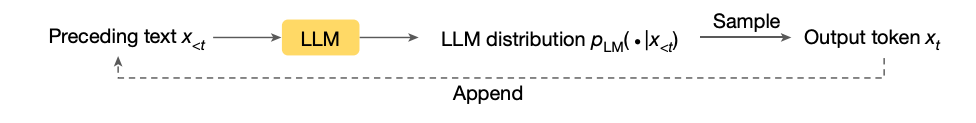
\includegraphics[width=0.8\textwidth]{figs/bg_autoregressive.png}
    \end{figure}
    \begin{itemize}
        \item Example:
    \end{itemize}
    \begin{figure}
        \centering
        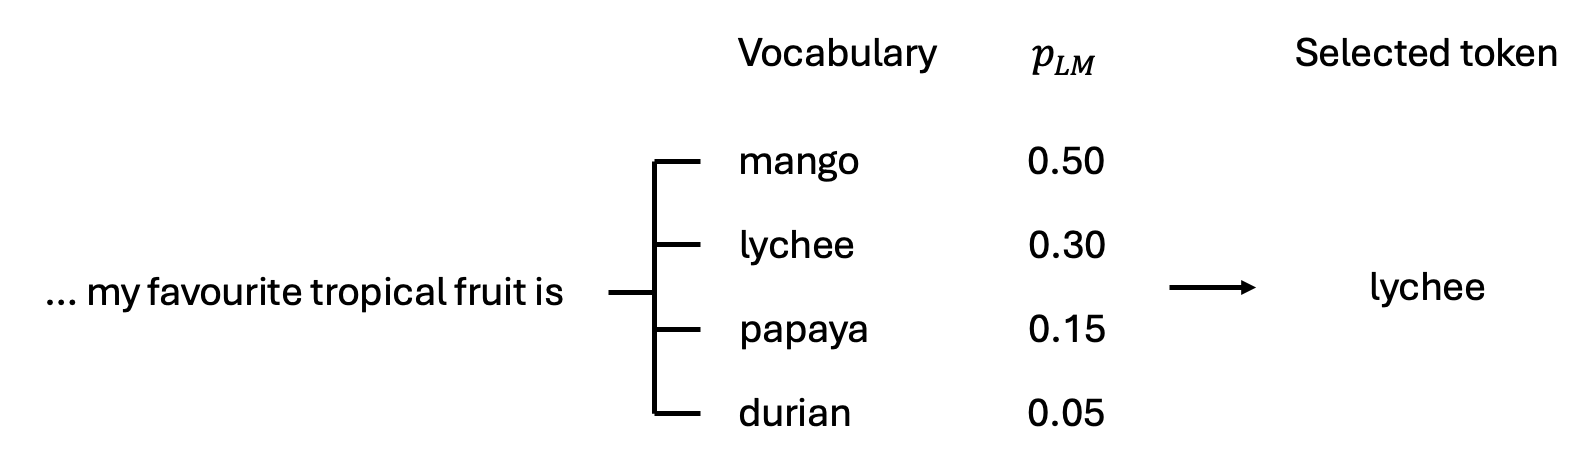
\includegraphics[width=0.6\textwidth]{figs/bg_autoreg_example.png}
    \end{figure}
\end{frame}

\begin{frame}[t]{Existing Approaches for LLM Text Detection}
    \begin{figure}
        \centering
        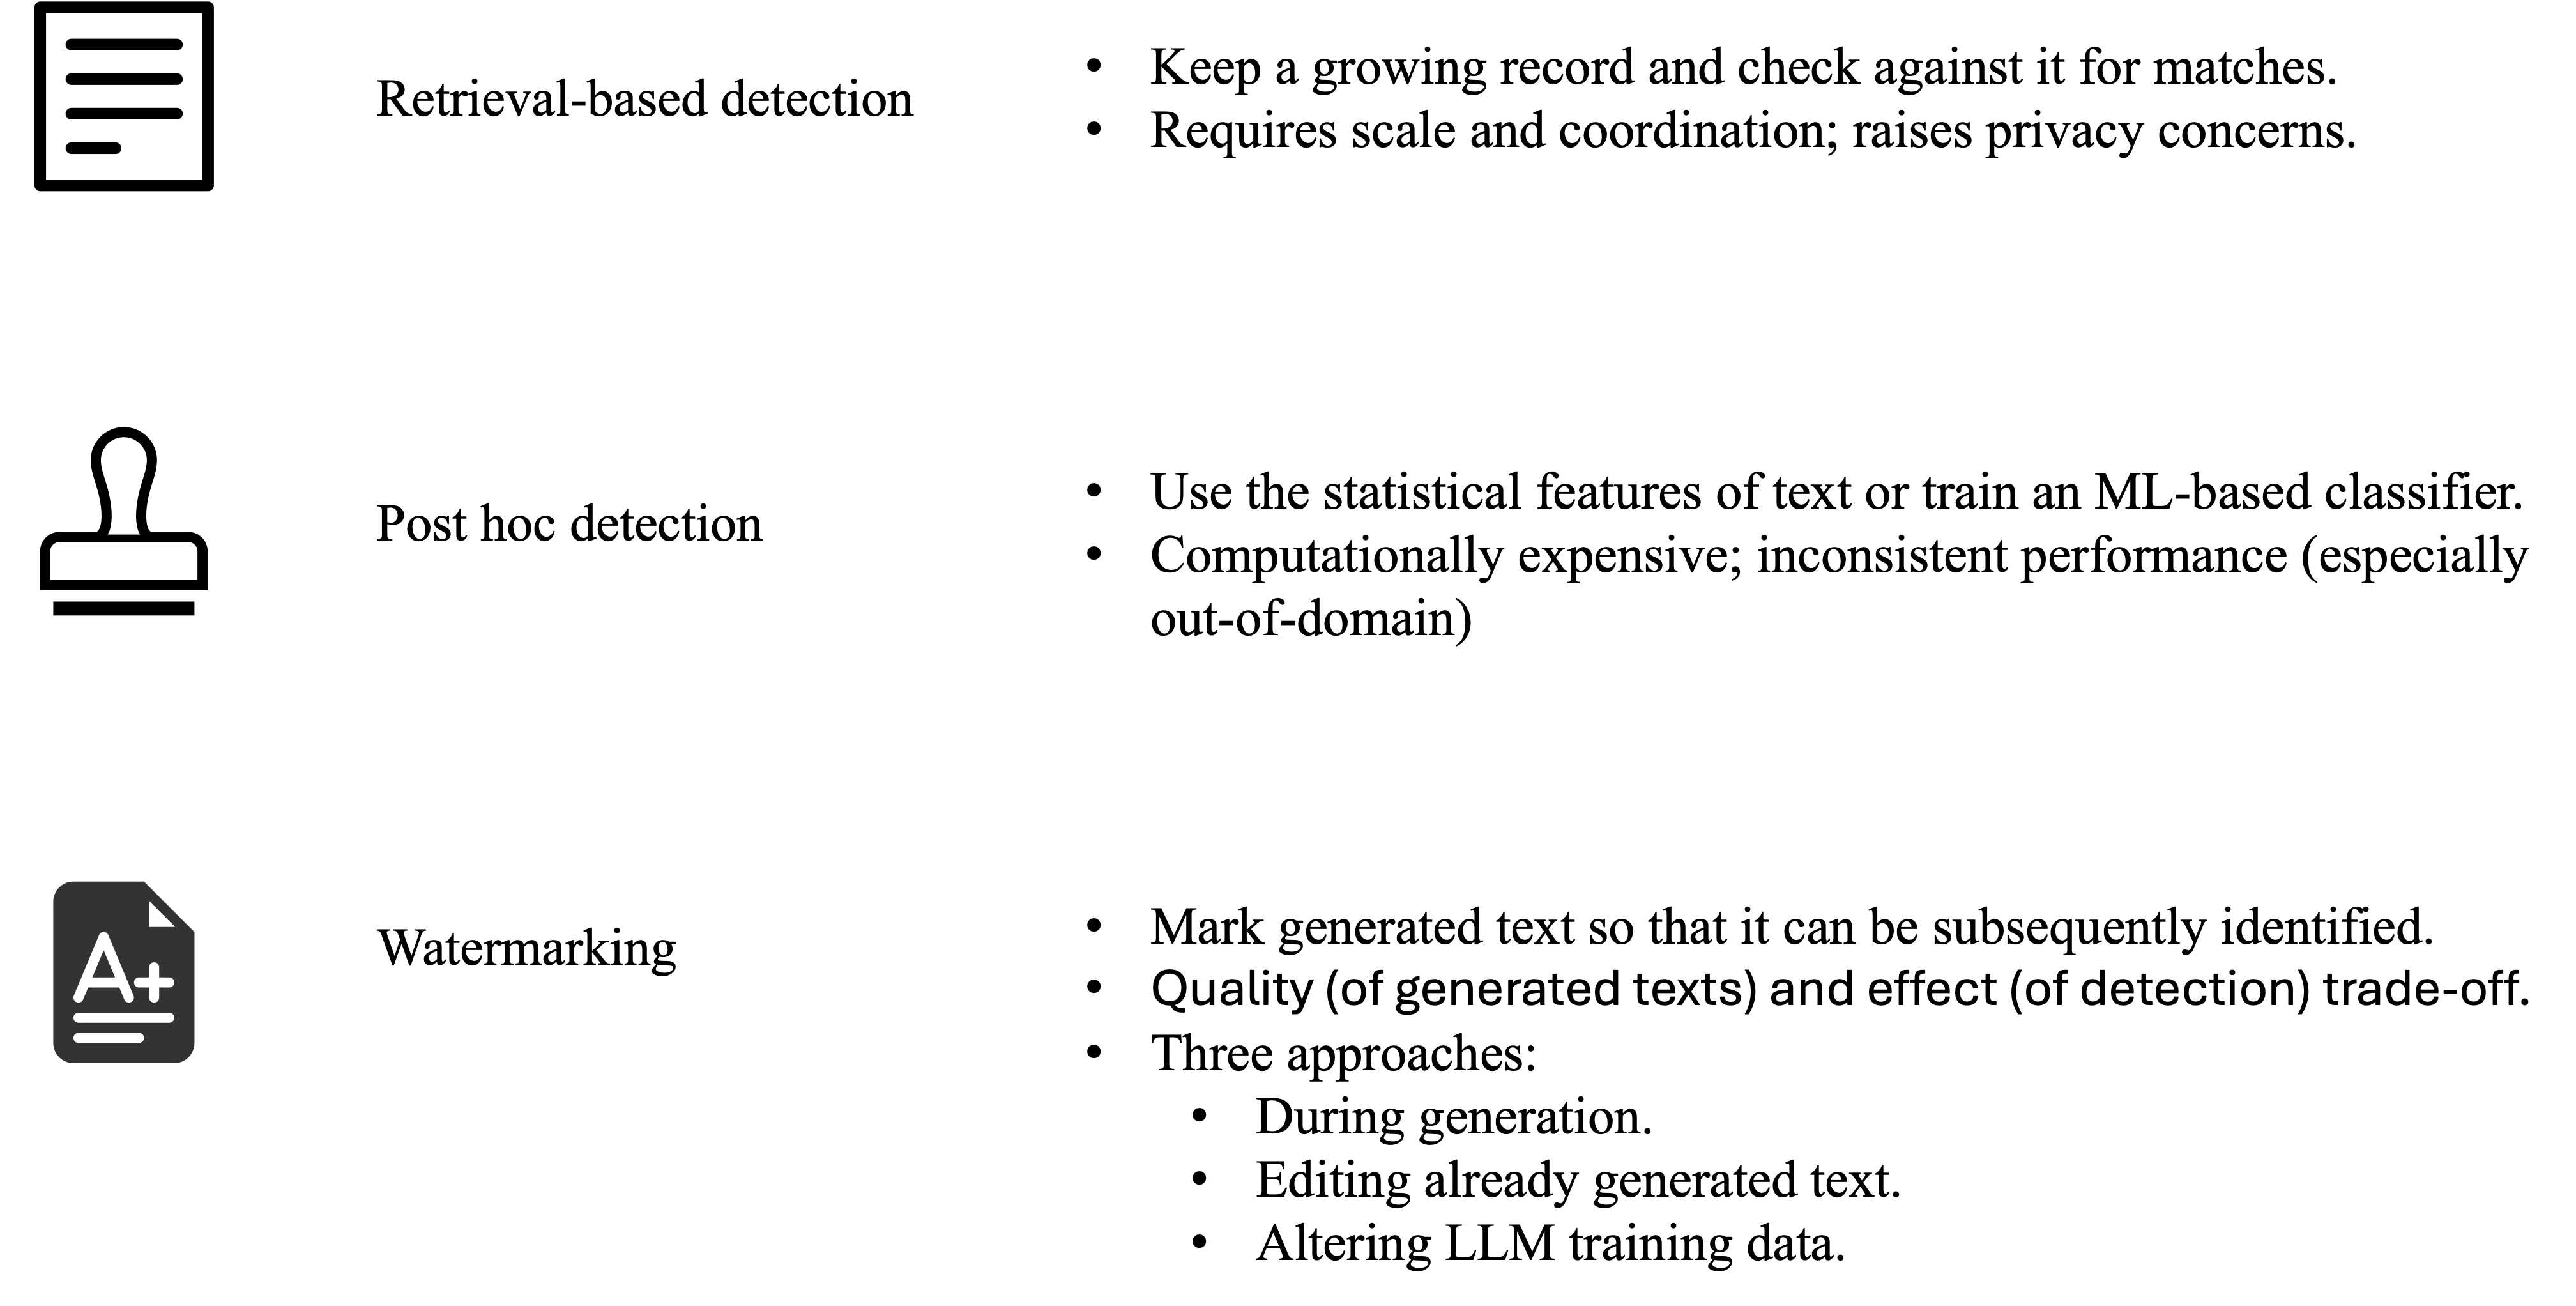
\includegraphics[width=0.9\textwidth]{figs/bg_summary.png}
    \end{figure}
\end{frame}

\begin{frame}[t]{Existing Approaches for LLM Text Detection}
    \begin{figure}
        \centering
        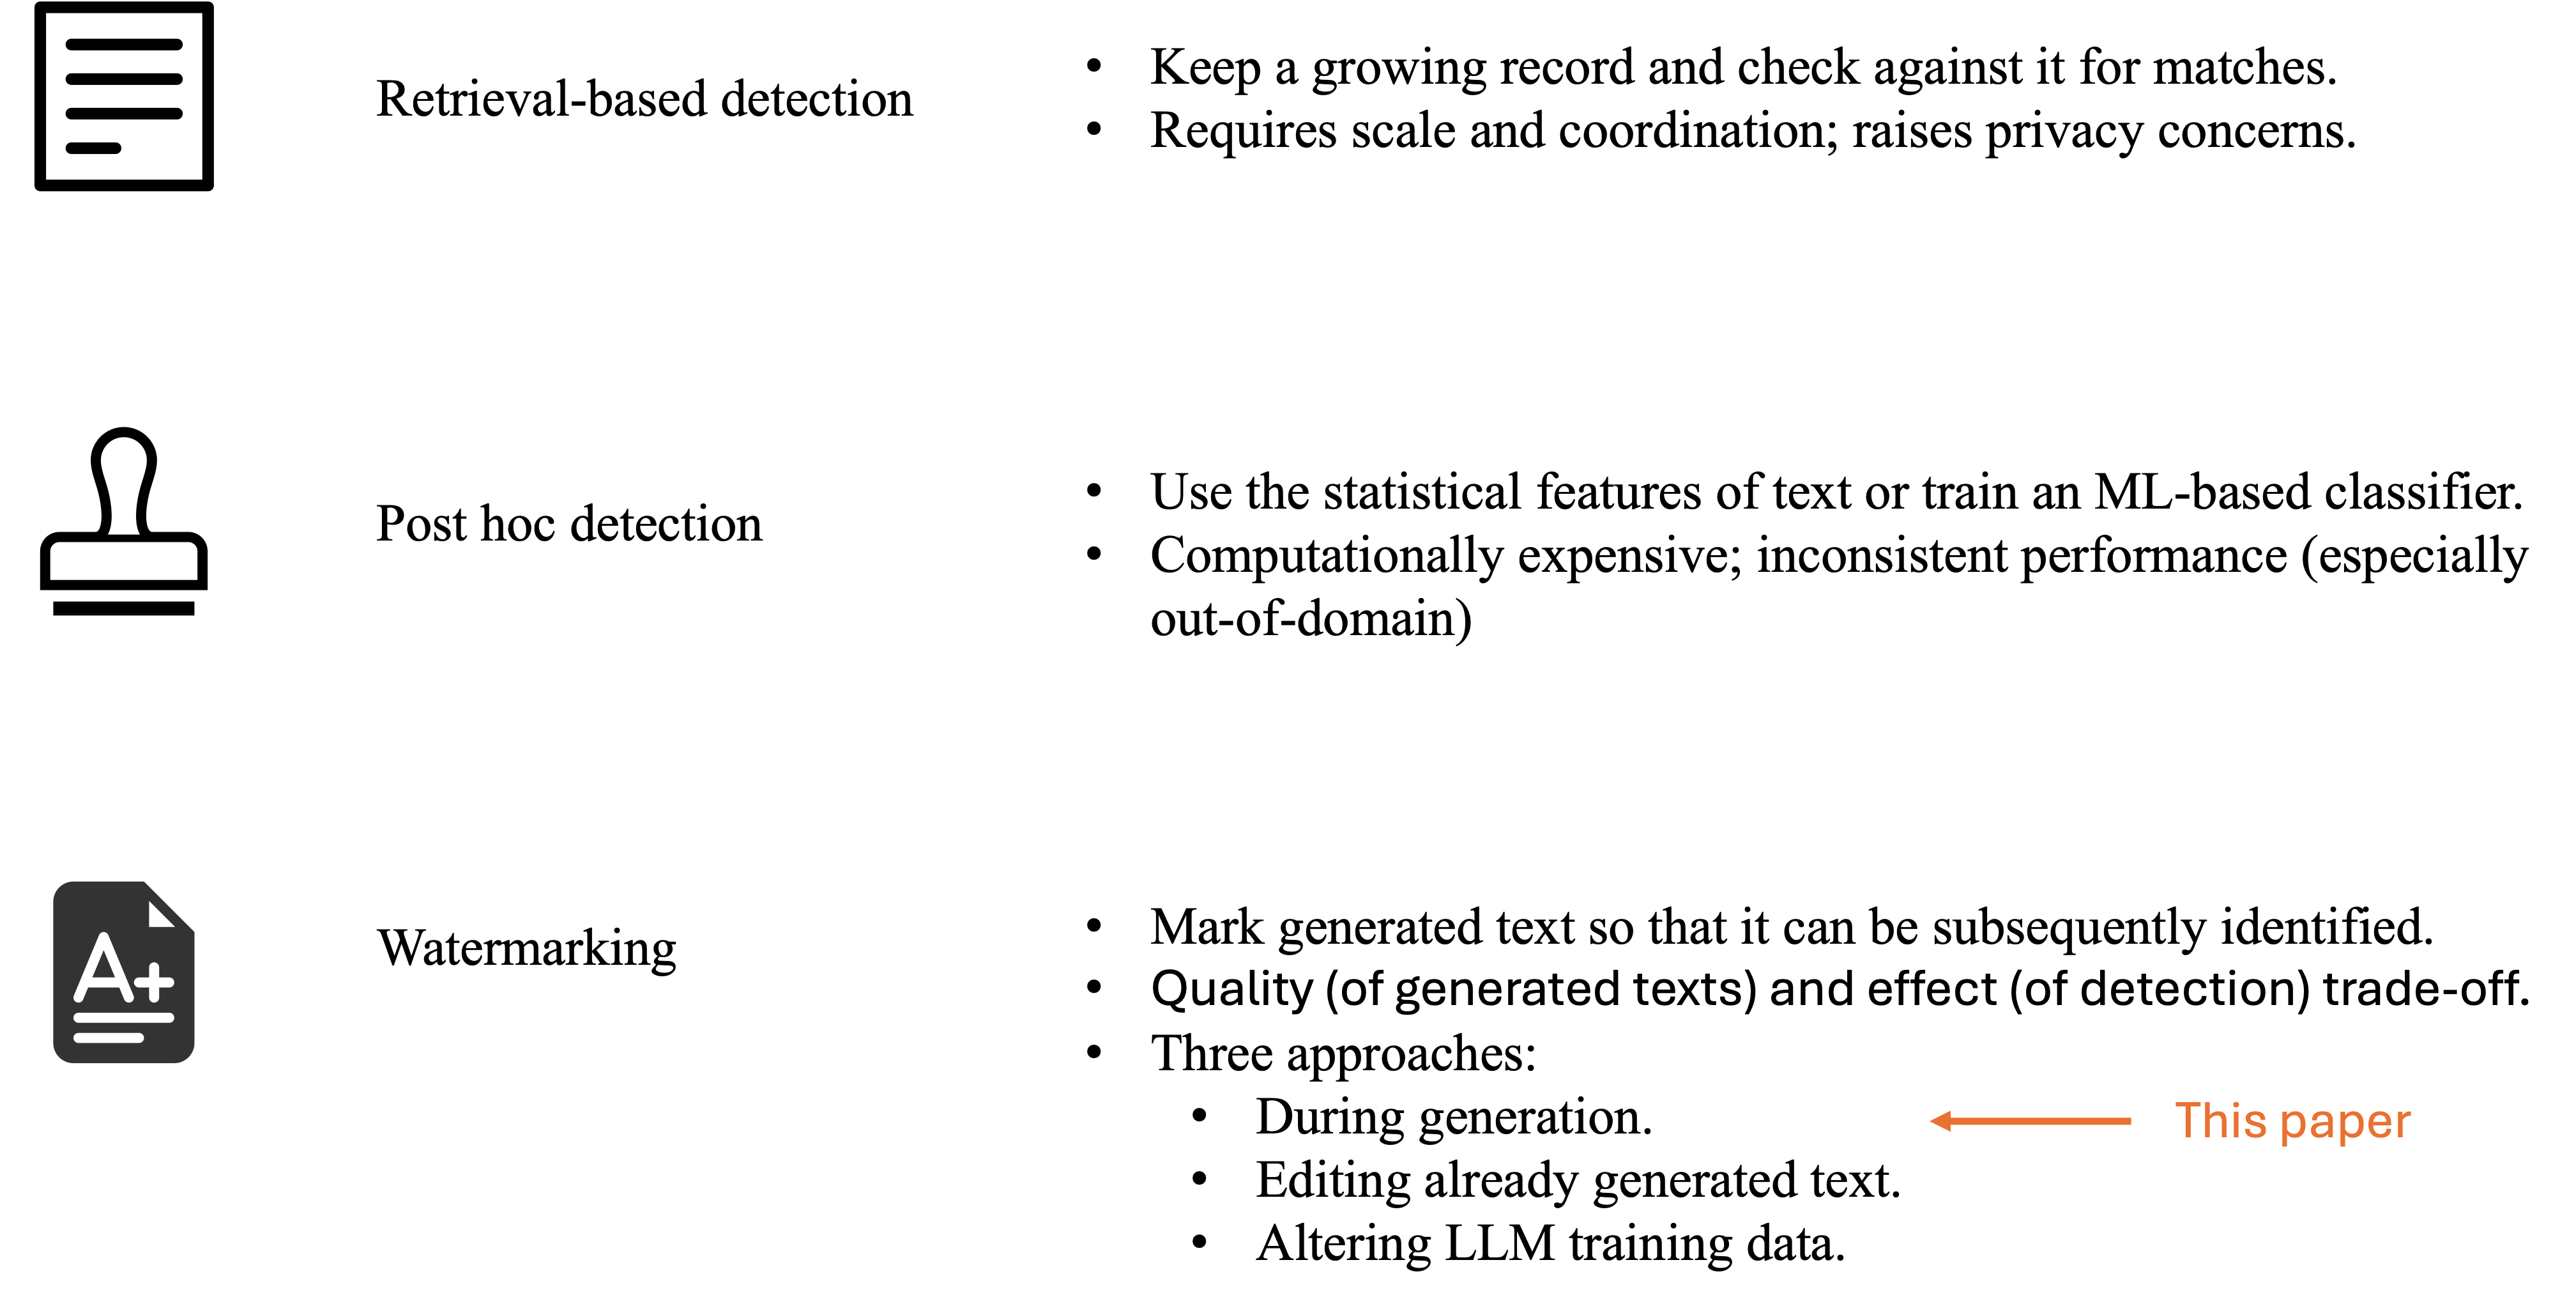
\includegraphics[width=0.9\textwidth]{figs/bg_summary2.png}
    \end{figure}
\end{frame}


\begin{frame}[t]{Intuition behind watermarking -- Monopoly}
    \begin{center}
        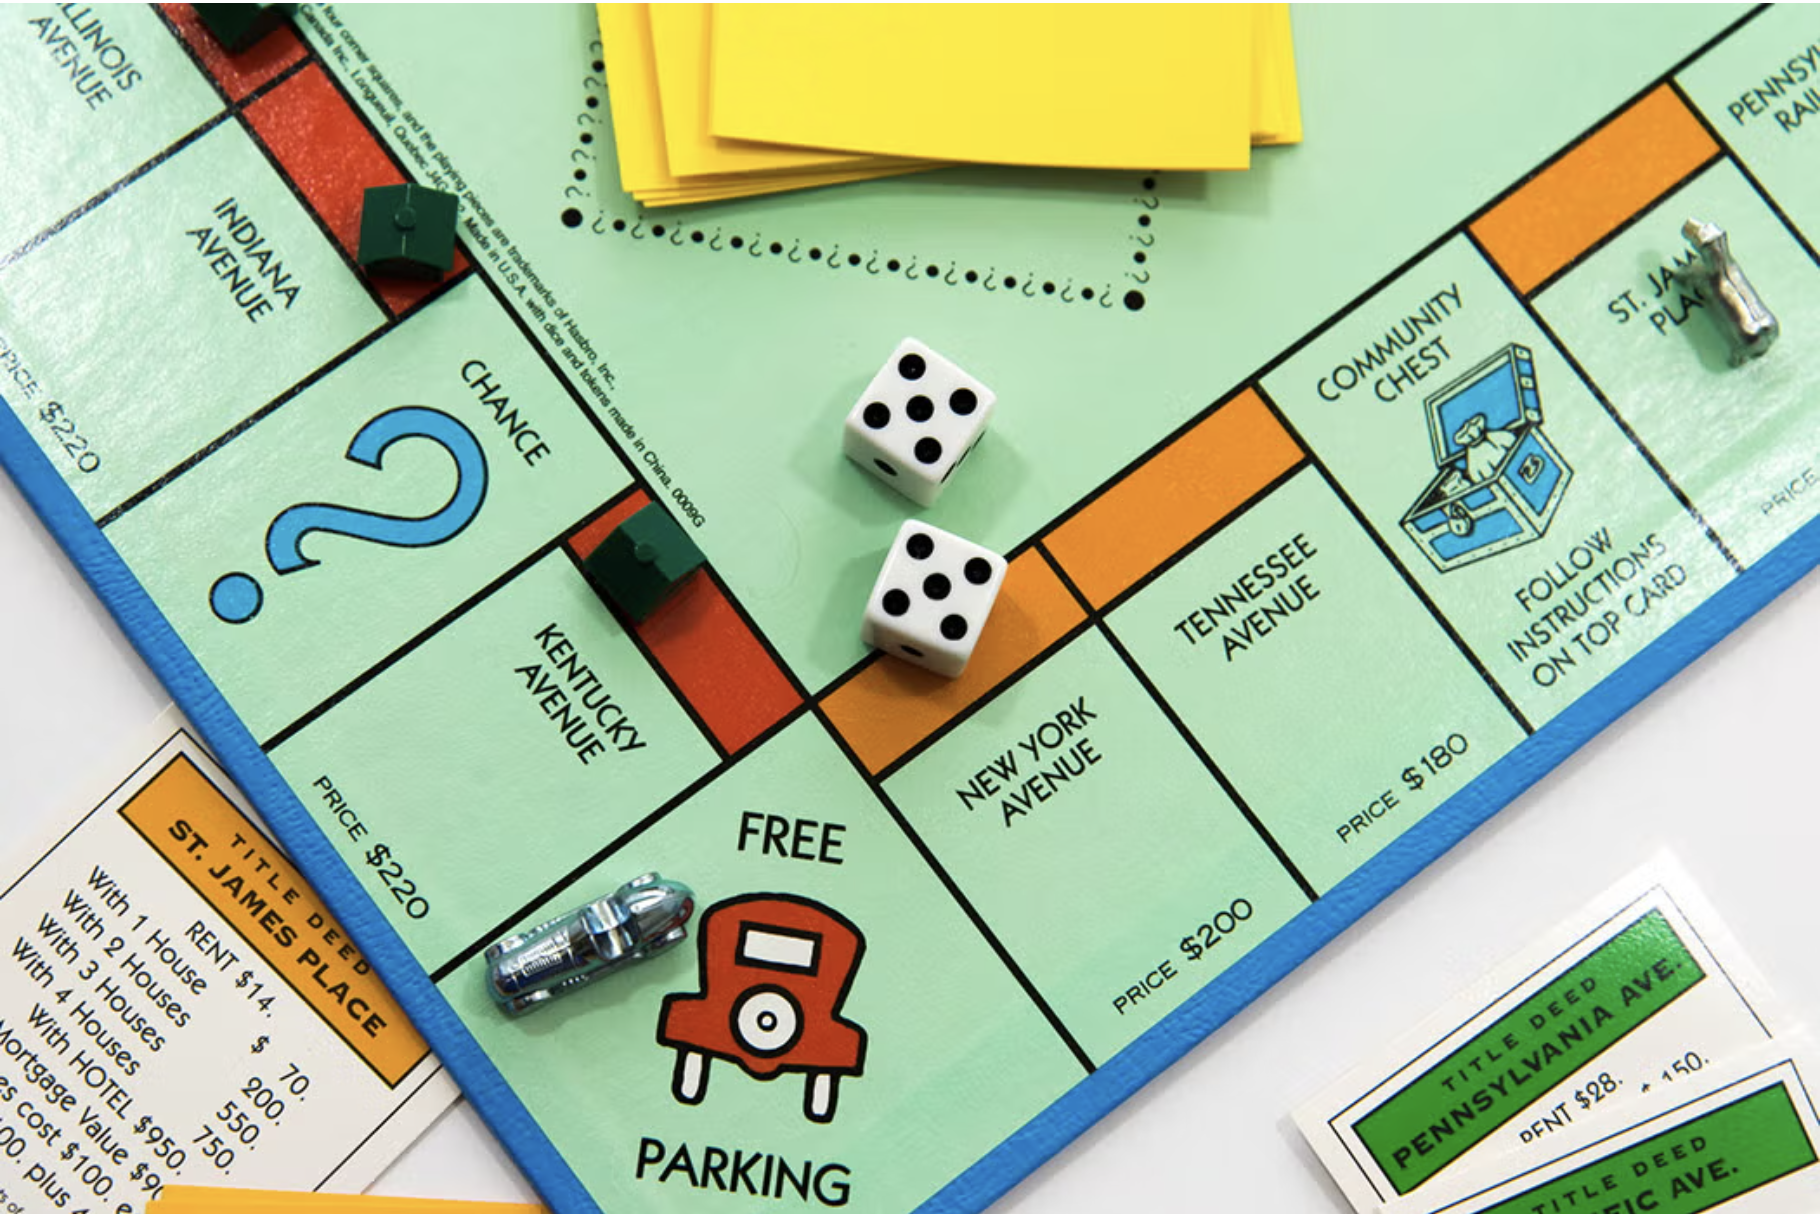
\includegraphics[width=0.4\textwidth]{figs/bg_monopoly.png}
    \end{center}

    \begin{itemize}
        \item[\raisebox{-0.4\height}{
\includegraphics[width=1.2em]{figs/bg_dice.png}}]
              Method 1: roll a dice
        \item[\raisebox{-0.4\height}{
\includegraphics[width=1.2em]{figs/bg_pi.png}}]
              Method 2: book of $\pi$ (3.1415926\textcolor{orange}{5358979323846...})
    \end{itemize}

    \begin{block}{}
        Both are random, but Method 2 is back-traceable (watermarked).
    \end{block}
\end{frame}

\section{SynthID-Text}
\begin{frame}[t]{}
    \vfill
    \begin{itemize}
        \item \url{https://github.com/google-deepmind/synthid-text}
        \item \url{https://watermark.keito.me/}
    \end{itemize}
    \vfill
\end{frame}


\begin{frame}[t]{SynthID-Text overview}
    \begin{figure}
        \centering
        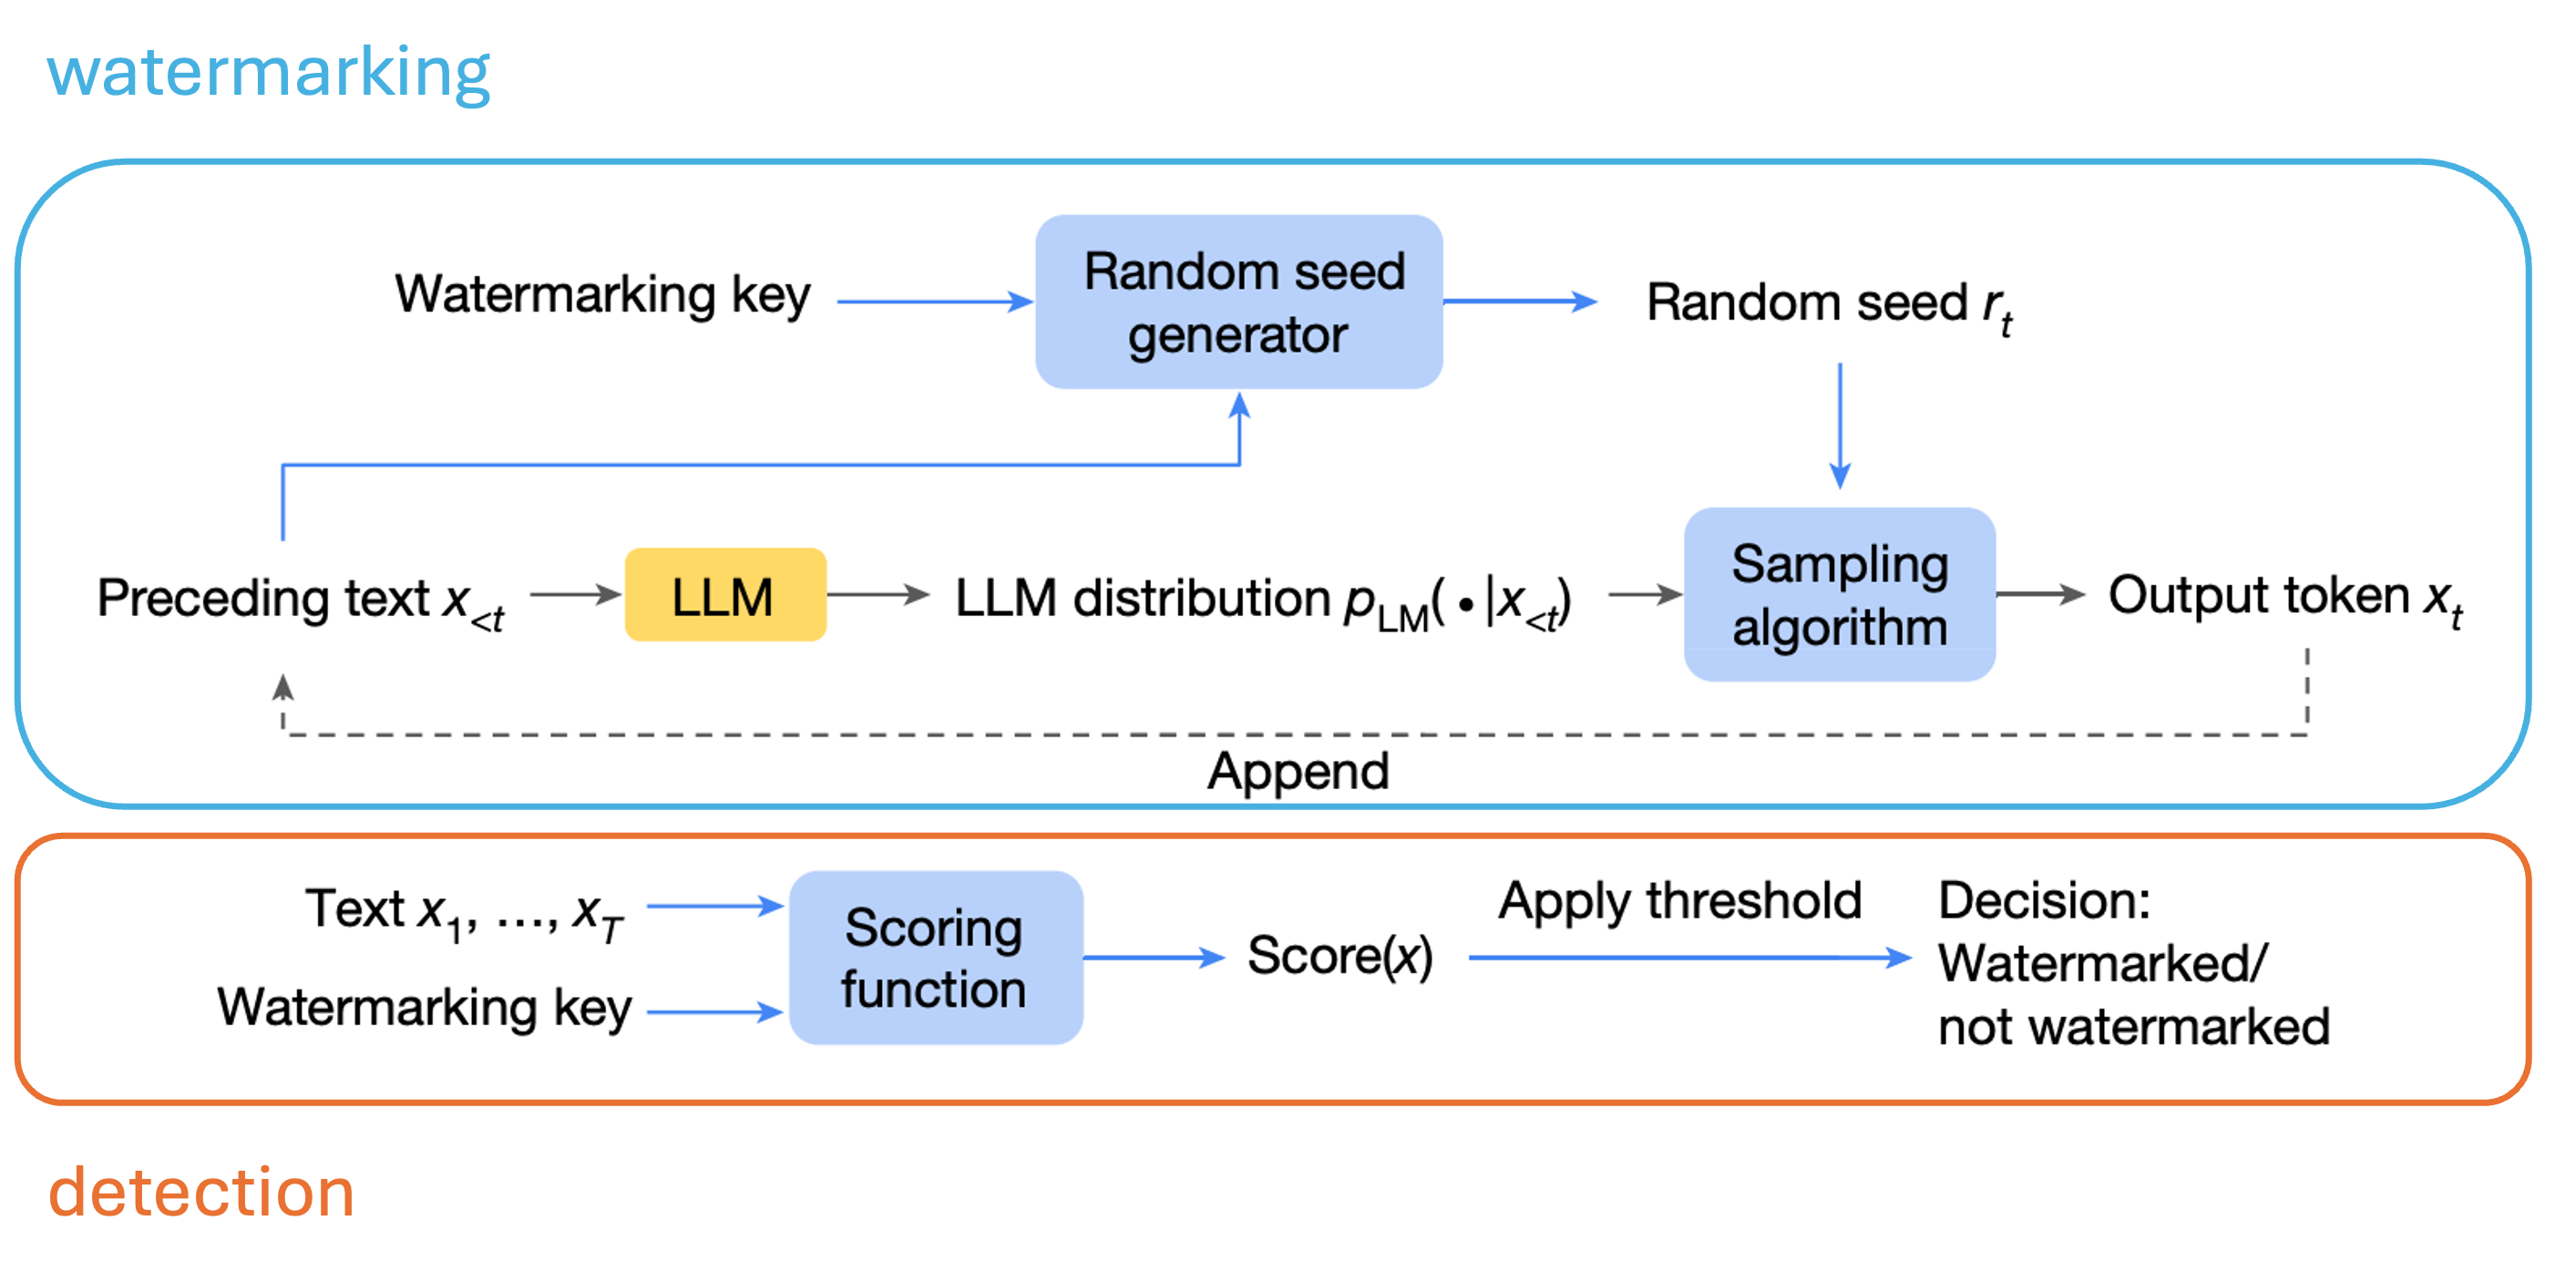
\includegraphics[width=0.7\textwidth]{figs/method_overview.png}
    \end{figure}

    \begin{itemize}
        \item Non-distortionary.
        \item Computationally efficient.
    \end{itemize}

    \vfill

    \sourcenote{Fig.~1, Dathathri et al.}
\end{frame}

\begin{frame}[t]{Watermarking -- Tournament Sampling}
    \focus{Tournament Sampling}: use a tournament-like process to select a token from the LLM distribution that is likely to score higher under some random watermarking functions.

    \begin{figure}
        \centering
        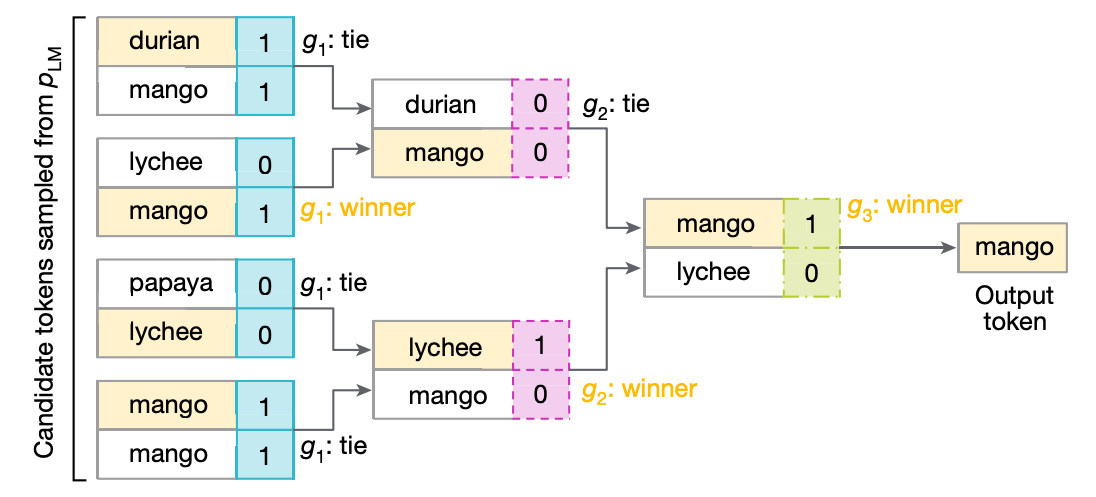
\includegraphics[width=0.6\textwidth]{figs/method_tournament_sampling.png}
    \end{figure}

    \focus{Watermarking function}: $g_l(x_t, r_t)$, where $x_t$ is a candidate token, and $r_t$ is a random seed.

    \begin{itemize}
        \item Number of layers $m$. Larger $m$ $\rightarrow$ better detectability. They use $m = 30$.
        \item Number of candidates $N$. Larger $N$ $\rightarrow$ better detectability. They use $N = 2$.
    \end{itemize}
\end{frame}

\begin{frame}[t]{Watermarking function}
    \vfill
    \begin{example}[binary watermarking function]
        $g_l(x, r) = \ind\{u_l(x, r) > 0.5\}$, where 
        \begin{align*}
            u_l(x, r) = \frac{h(x, r, l)}{2^{n_{\text{sec}}}} \;\in\; [0, 1) \;,
        \end{align*}
        $h$ is a pseudorandom function producing uniform-looking integers, and $n_{\text{sec}}$ is the security parameter.
    \end{example}
    \vfill
    
\end{frame}

\begin{frame}[t]{Watermarking detection \gray{(Appendix A)}}
    \begin{align*}
        \mathrm{Score}(x) = \frac{1}{mT} \sum_{t=1}^T \sum_{l=1}^m g_l(x_t, r_t) \;.
    \end{align*}
    
    \begin{block}{}
        Intuition: $\mathrm{Score}(x)$ takes higher values for a watermarked sequence.
    \end{block}

    Context index $t$ is only summed over a subset $\hat{T} \subseteq \{1, \ldots, T\}$ that
    \begin{itemize}
        \item excludes the first $t = 1, \ldots, H$ tokens, where the context window is incomplete.
        \item excludes $t$ where the context $x_{t-H}, \ldots, x_{t-1}$ has appeared previously in the sequence.
    \end{itemize}

    \begin{example}[$H = 3$]
        {\footnotesize
        "$\underbrace{\textcolor{red}{\text{Explain in one}}}_{\text{\scriptsize incomplete}}$ short paragraph how to come up with nice banters \underline{for machine learning} talks tailored $\underbrace{\textcolor{orange}{\text{for machine learning}}}_{\text{\scriptsize repeated}}$ experts."
        }
    \end{example}

\end{frame}

\begin{frame}[t]{Watermarking detection \gray{(Appendix A)}}
    \vfill
    \begin{block}{Hypothesis testing for watermarking}
        Under 
        \begin{align*}
            H_0: \text{the text is not watermarked by SynthID-Text} \;,
        \end{align*}
        each $g_l(x_t, r_t)$ is i.i.d., and the $p$-value of $\mathrm{Score}(x)$ has an explicit form.
    \end{block}
    \vfill
\end{frame}

\begin{frame}[t]{Quality preservation \gray{(Appendix G)}}

    \begin{block}{In words}
        A sampling algorithm is non-distortionary if in expectation the distribution on the next token is identical before and after watermarking.
    \end{block}
    
    \begin{figure}
        \centering
        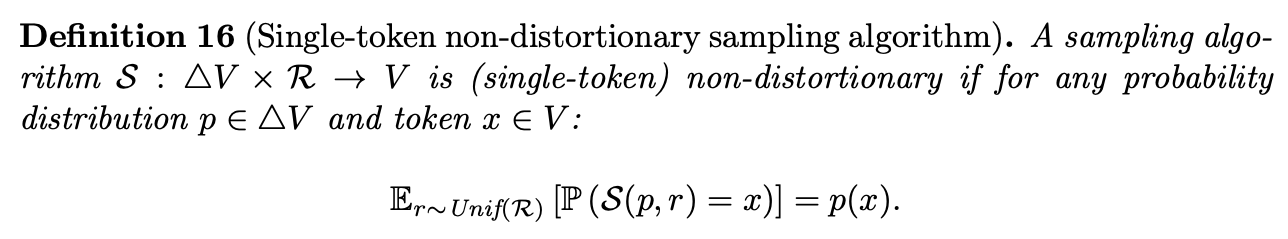
\includegraphics[width=0.9\textwidth]{figs/method_non_distort.png}
    \end{figure}
    {\footnotesize
    \begin{itemize}
        \item $V = $ set of candidate tokens.
        \item $\Delta V = \text{probability simplex over $V$} = \{ p: V \rightarrow [0, 1] \mid \sum_{x \in V} p(x) = 1 \}$. 
        \item $\mathcal{R} = $ set of possible random seeds.
    \end{itemize}
    }

\end{frame}

\begin{frame}[t]{Qualifty preservation \gray{(Appendix G)}}

    \vfill

    \focus{$K$-sequence non-distortion}: a stronger version of single-token non-distortion that holds for \textbf{sequences} of tokens.

    \begin{block}{\bf{Theorem 21}}
        For any $K \geq 1$, SynthID-Text \gray{(with $N=2$ and $K$-sequence repeated context masking)} is $K$-sequence non-distortionary.
    \end{block}

    \vspace{2em}
    \begin{example}[$K$-sequence repeated context masking, $K=2$]
        "Explain in one short paragraph how to come up with nice banters \underline{for machine learning} talks tailored \textcolor{orange}{for machine learning} experts."

        "Give me a concrete example of a joke \textcolor{orange}{for machine learning} that I can use to start my talk."

    \end{example}
    \vfill
\end{frame}


\begin{frame}[t]{Computational complexity}
    
    \begin{table}
        \centering
        \begin{tabular}{lrr}
            \hline
            Sampling method & Latency (ms/token) & Increase (\%) \\
            \hline
            Baseline                       & 15.527 & --    \\
            Tournament sampling ($m=30$ layers) & 15.615 & 0.57 \\
            Gumbel sampling                & --     & 0.26 \\
            Soft Red List                  & --     & 0.28 \\
            \hline
        \end{tabular}
        \caption{Gemma 7B-IT latency on 4 v5e TPUs.}
        \label{tab:watermark-latency}
    \end{table}
    
    \begin{block}{}
        SynthID-Text can be integrated into large-scale production systems with ``negligible additional computational overhead''.
    \end{block}

\end{frame}

\section{Empirical evaluation}
\begin{frame}[t]{Empirical evaluation -- scalability to number of tokens}

    \begin{figure}
        \centering
        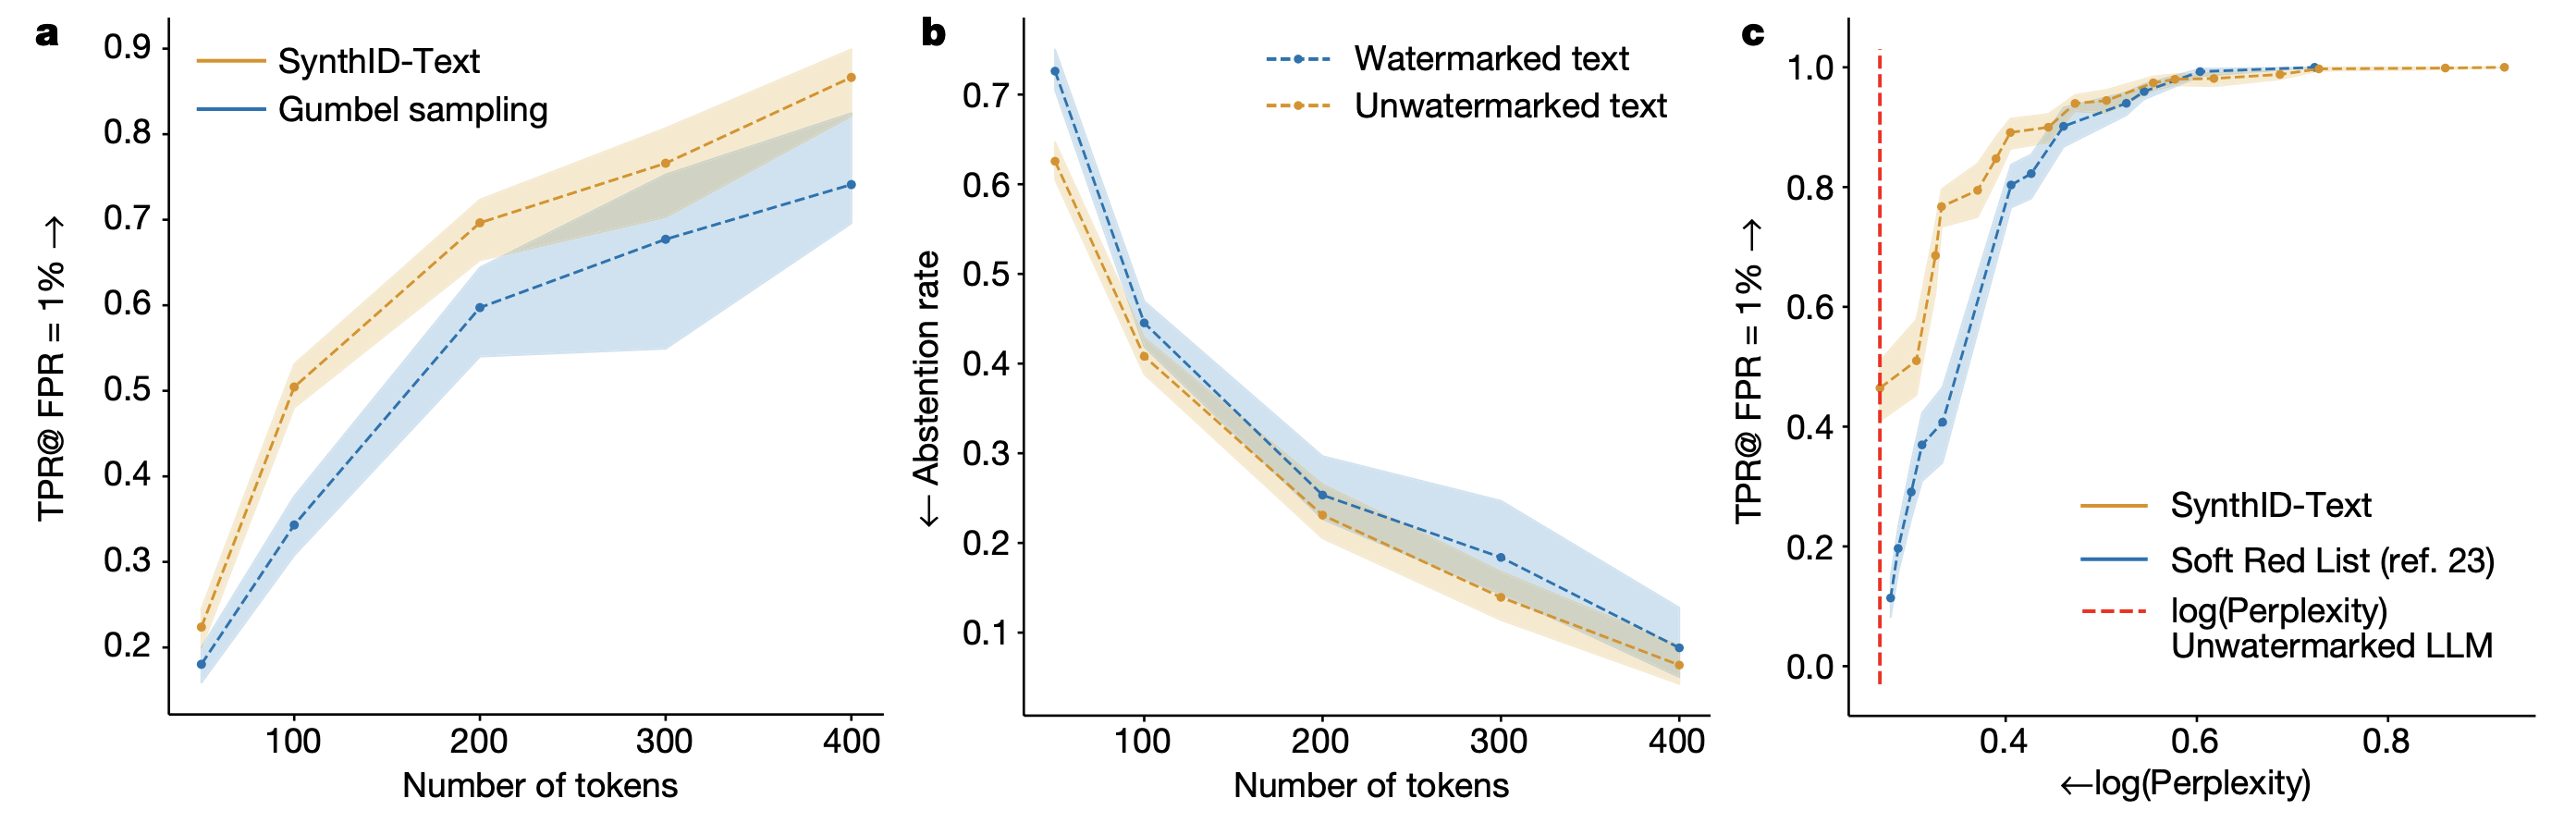
\includegraphics[width=0.8\textwidth]{figs/eval_detectability.png}
        \caption*{\textbf{Fig.3:} Detection performance of SynthID-Text, using prompts from the ELI5 dataset.}
    \end{figure}
\end{frame}

\begin{frame}[t]{Empirical evaluation -- scalability to $m$}
    \begin{figure}
        \centering
        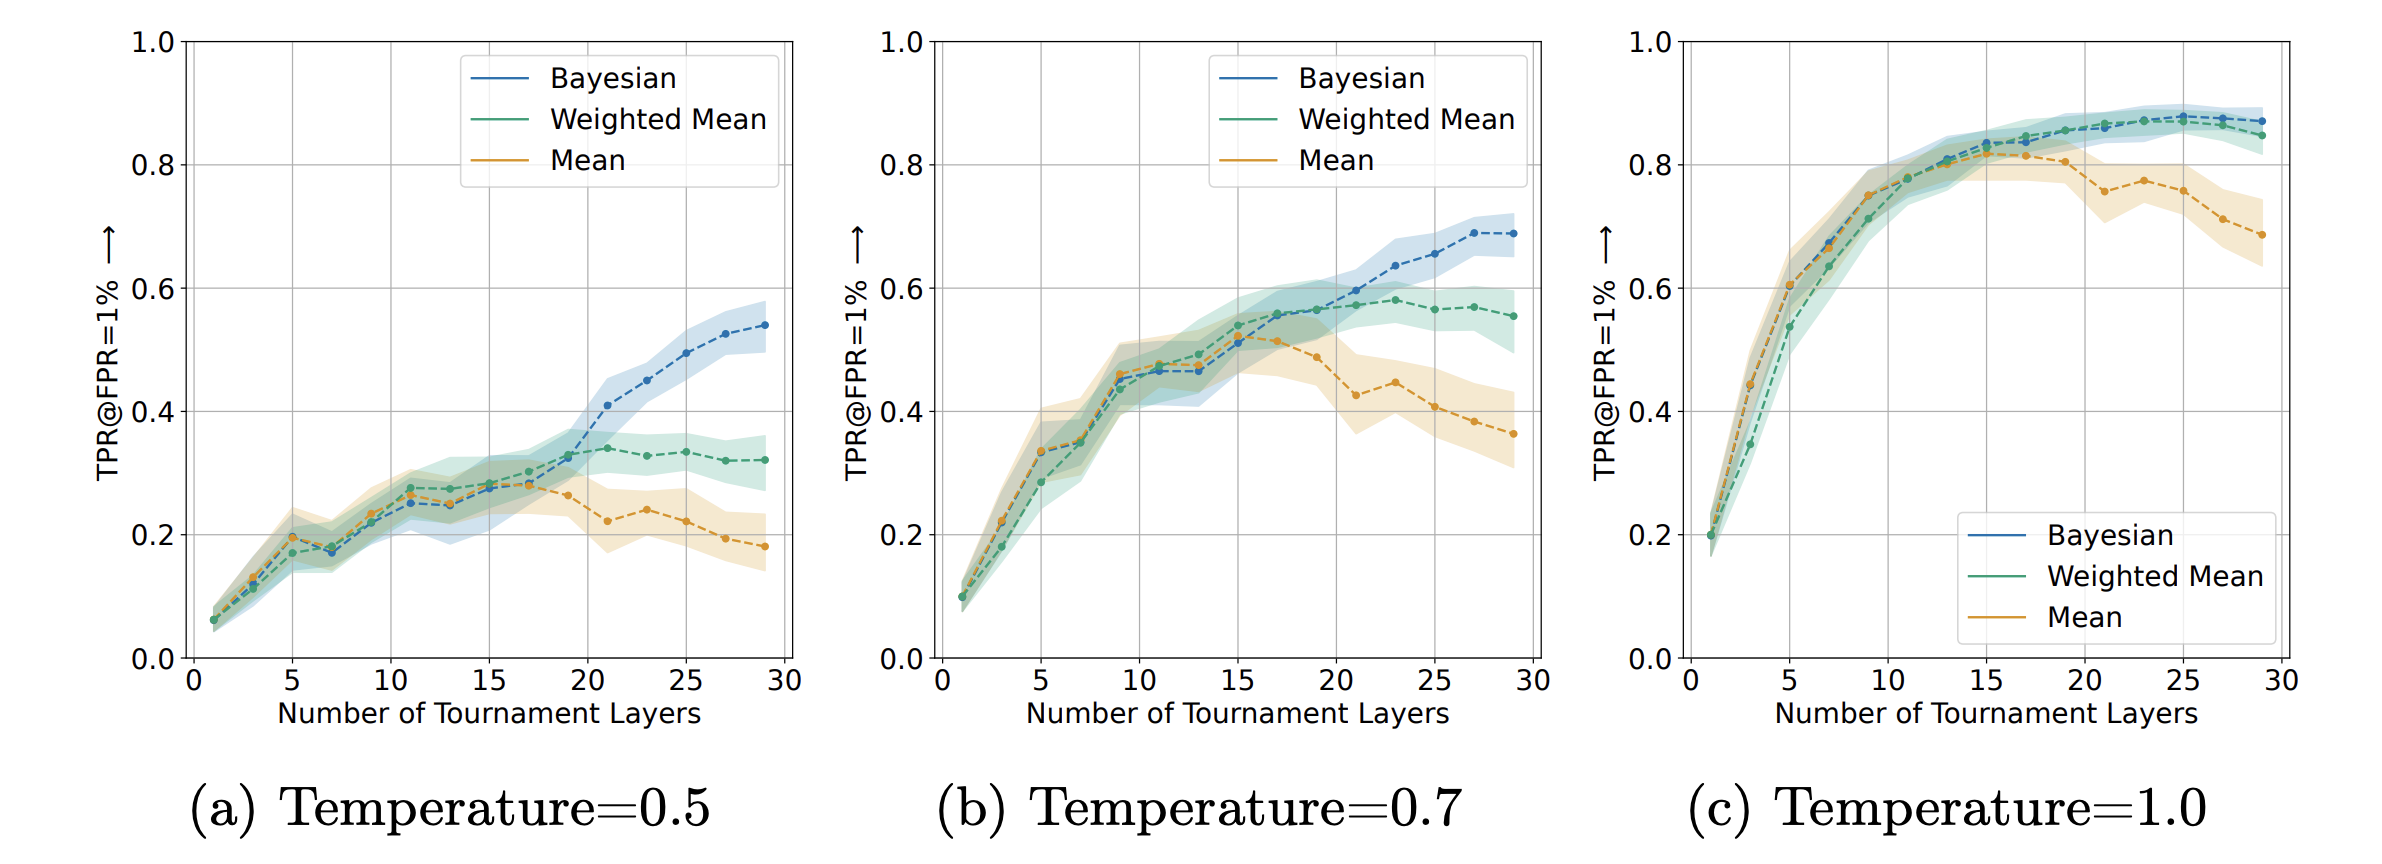
\includegraphics[width=0.8\textwidth]{figs/eval_effect_of_m.png}
        \caption*{\textbf{Fig.C1:} Detectability with respect to number of tournament layers $m$.}
    \end{figure}
\end{frame}

\begin{frame}[t]{Empirical evaluation -- robustness under perturbation}
    \begin{figure}
        \centering
        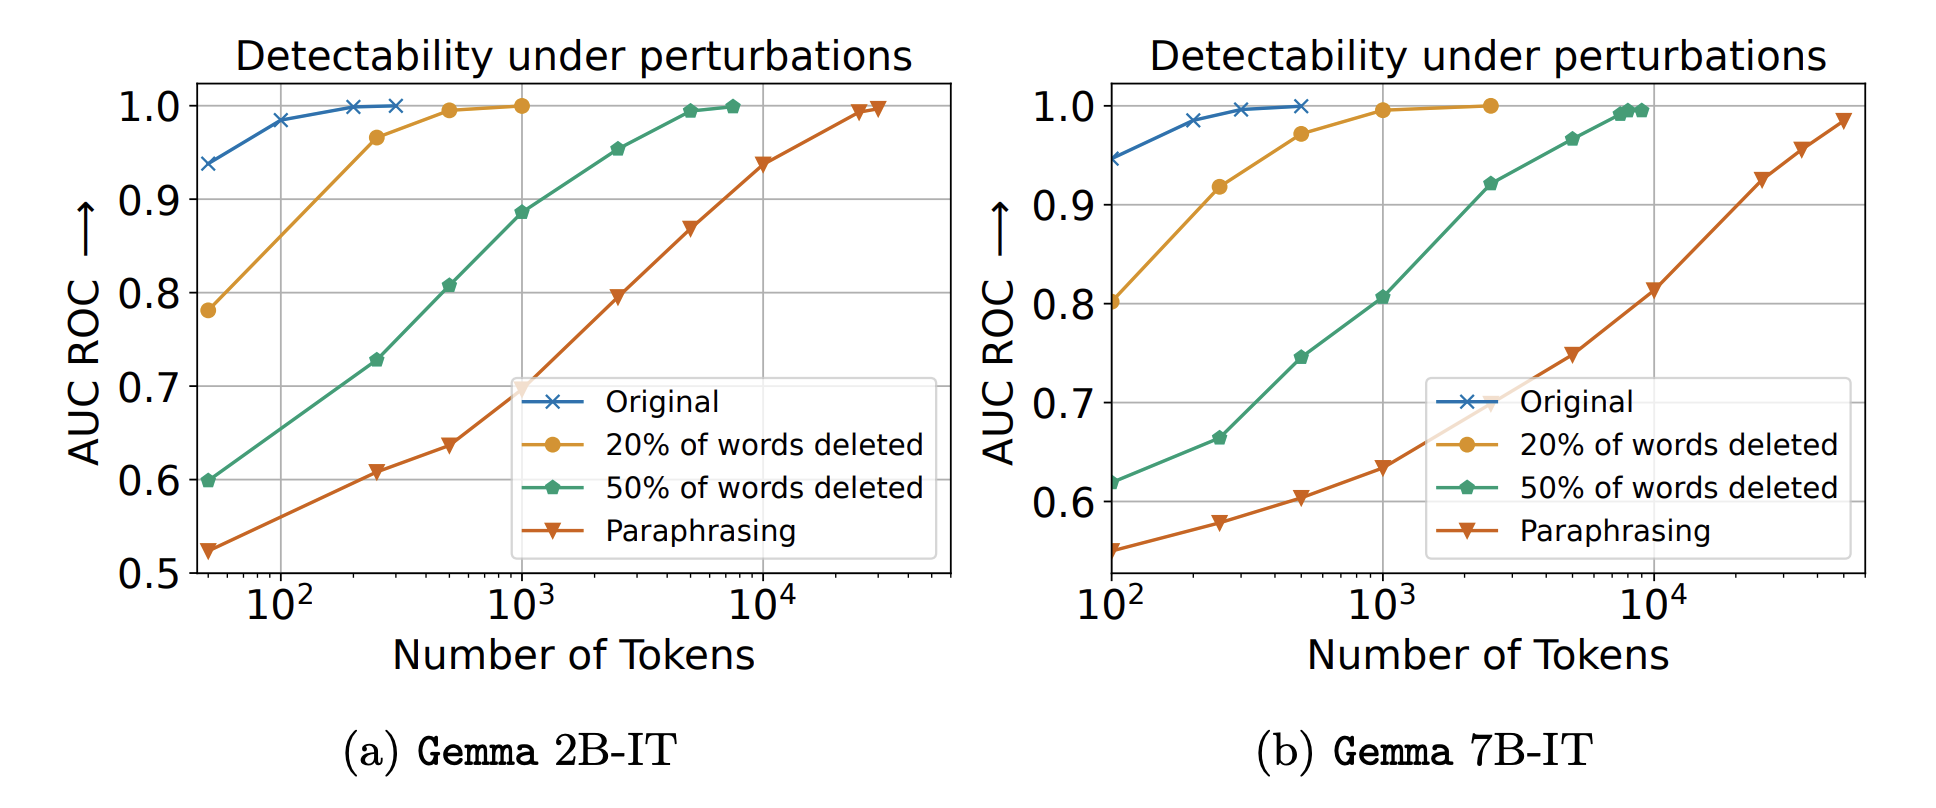
\includegraphics[width=0.8\textwidth]{figs/eval_robustness.png}
        \caption*{\textbf{Fig.C3:} Detectability under various perturbations.}
    \end{figure}
\end{frame}

\section{Discussion}
\begin{frame}[t]{Some remarks}
    \vfill
    \begin{itemize}
        \item \focus{Diversity}: Same diversity within a single text, but reduced diversity for the same prompt.
        \item \focus{Limitation}: Requires full knowledge of the watermarking scheme for the detection to work --- 
            \begin{itemize}
                \item NOT a generic LLM-content detector.
                \item Alternatives exist: \url{pangram.com}
            \end{itemize}
        \item \focus{Adversarial attacks}: Even a simple translation trick can be effective.
        \item \focus{Evaluation}: Various evaluation principles presented (frequentist, Bayesian, with/without perturbation). What is EU's rule?
    \end{itemize}
    \vfill
\end{frame}

\end{document}
